\usetikzlibrary{patterns.meta}
\begin{frame}[fragile]{UDP format}
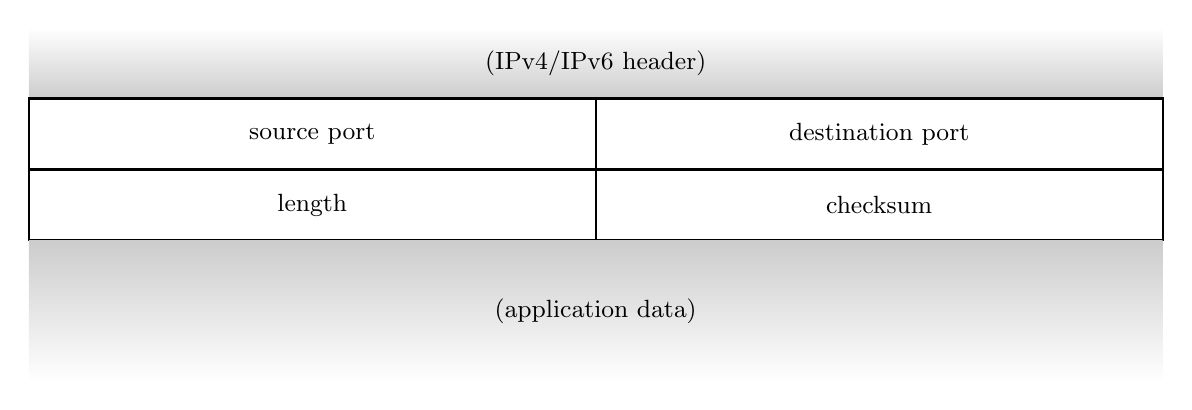
\begin{tikzpicture}
\tikzset{
    box/.style={draw,thick},
    label/.style={font=\small},
    label large/.style={},
    box label/.style={midway,font=\small,align=center},
    box label flags/.style={midway,font=\fontsize{8}{9}\selectfont,align=center},
    missing/.style={pattern=north west lines},
}
\begin{scope}[x=0.45cm,y=0.9cm]
\path[shading=axis,top color=white,bottom color=black!20] (0, 1) rectangle (32, 0)
    node[box label] {(IPv4/IPv6 header)};
\draw[box] (0, 0) rectangle (16, -1)
    node[midway,label] {source port};
\draw[box] (16, 0) rectangle (32, -1)
    node[midway,label] {destination port };
\draw[box] (0, -1) rectangle (16, -2)
    node[midway,label] {length};
\draw[box] (16, -1) rectangle (32, -2)
    node[midway,label] {checksum};
\path[shading=axis,bottom color=white,top color=black!20] (0, -2) rectangle (32, -4)
    node[box label] {(application data)};
\end{scope}
\end{tikzpicture}
\end{frame}
